% Number 500
% CAPMA CVPMA 
% Stoplight stopping
% KO

% Watermark
\AddToShipoutPicture*{\BackgroundPic}

\addtocounter {ProbNum} {1}

%\begin{floatingfigure}[r]{.33\textwidth}
%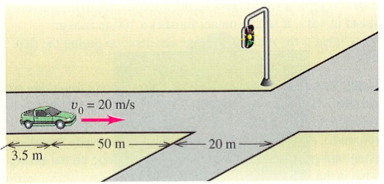
\includegraphics[scale=.6]{/Users/jgates/desktop/latex/pics/redlight}
%\end{floatingfigure}
 
{\bf \Large{\arabic{ProbNum}}} A car 3.5 m in length and traveling at a constant speed of ${20~\tfrac{m}{s}}$ is approaching an intersection. The width of the intersection is 20 m. The light turns yellow when the front of the car is 50 m from the beginning of the intersection. If the driver steps on the brake, the car will slow at a rate of ${4.2~\tfrac{m}{s}}$ per second. If the driver instead steps on the gas pedal, the car will accelerate at ${1.5~\tfrac{m}{s^2}}$. The light will be yellow for 3 seconds. Ignore the reaction time of the driver. 

\bigskip
To avoid being in the intersection while the light is red, should the driver hit the brake pedal or the gas pedal? Justify your answer with some pretty physics.

\hfill 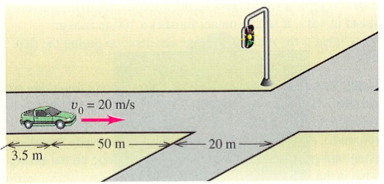
\includegraphics[scale=.85]{/Users/jgates/desktop/latex/pics/redlight.png}


\vfill
\newpage
